\documentclass[11pt,a4paper]{article}

\usepackage[utf8]{inputenc}
\usepackage[T1]{fontenc}
\usepackage{lmodern}
\usepackage[a4paper,margin=1in]{geometry}
\usepackage{amsmath, amssymb}
\usepackage{longtable}
\usepackage{array}
\usepackage{booktabs}
\usepackage{listings}
\usepackage{graphicx}
\usepackage{tabularx}
\usepackage{xcolor}
\usepackage{enumitem}
\usepackage{titlesec}
\usepackage{float}
\usepackage[hypertexnames=false]{hyperref}
\usepackage[protrusion=true,expansion=false]{microtype}
\usepackage{fancyhdr}
\usepackage[font=small,labelfont=bf]{caption}
\usepackage{url}
\usepackage{xurl}
\usepackage{cite}

% Listings configuration (Verilog/Python/ASM support)

% ---- Color palette ----
\definecolor{codebg}{RGB}{248,248,248}
\definecolor{codeframe}{RGB}{220,220,220}
\definecolor{codekw}{RGB}{0,92,184}
\definecolor{codestr}{RGB}{163,21,21}
\definecolor{codecom}{RGB}{0,128,0}
\definecolor{codenums}{RGB}{120,120,120}

% ---- Verilog language
% NOT: use language=Verilog
\lstdefinelanguage{Verilog}{
  morekeywords={
    always,and,assign,automatic,begin,buf,bufif0,bufif1,case,casex,casez,
    cell,config,deassign,default,defparam,design,disable,edge,else,end,
    endcase,endconfig,endfunction,endgenerate,endmodule,endprimitive,endspecify,
    endtable,endtask,event,for,force,forever,fork,function,generate,genvar,
    if,ifnone,initial,inout,input,integer,join,large,localparam,macromodule,
    medium,module,nand,negedge,nmos,nor,not,notif0,notif1,or,output,
    parameter,pmos,posedge,primitive,pull0,pull1,pulldown,pullup,rcmos,real,
    realtime,reg,release,repeat,rnmos,rpmos,rtran,rtranif0,rtranif1,scalared,
    signed,small,specify,specparam,strength,supply0,supply1,table,task,time,
    tran,tranif0,tranif1,tri,tri0,tri1,triand,trior,trireg,unsigned,
    vectored,wait,wand,while,wire,wor,xnor,xor,
    logic,bit,byte,shortint,int,longint,struct,union,enum,typedef,package,
    import,export,class,interface,modport,program,clocking,property,sequence,
    assert,assume,cover,final,unique,priority
  },
  sensitive=true,
  morecomment=[l]{//},
  morecomment=[s]{/*}{*/},
  morestring=[b]",
  alsoletter={_,$},
}

% consistent style used across the report
\lstdefinestyle{grstyle}{
  backgroundcolor=\color{codebg},
  basicstyle=\ttfamily\small,
  frame=single,
  rulecolor=\color{codeframe},
  frameround=tttt,
  framesep=6pt,
  xleftmargin=2.2em,
  framexleftmargin=2.2em,
  aboveskip=1.0em,
  belowskip=1.0em,
  breaklines=true,
  breakatwhitespace=true,
  columns=fullflexible,
  keepspaces=true,
  showstringspaces=false,
  tabsize=4,
  numbers=left,
  numberstyle=\scriptsize\color{codenums},
  numbersep=10pt,
  keywordstyle=\bfseries\color{codekw},
  commentstyle=\itshape\color{codecom},
  stringstyle=\color{codestr},
  captionpos=b,
  upquote=true,
  literate={→}{{$\to$}}1 {≤}{{$\le$}}1 {≥}{{$\ge$}}1 {≠}{{$\ne$}}1
}

% Default style
\lstset{style=grstyle}

\definecolor{accent}{RGB}{0,92,184}

\hypersetup{
    colorlinks=true,
    linkcolor=blue!60!black,
    citecolor=blue!60!black,
    urlcolor=blue!60!black
}

\setlist[itemize]{topsep=0.35em,itemsep=0.2em}
\setlist[enumerate]{topsep=0.35em,itemsep=0.2em}

\titleformat{\section}
    {\Large\bfseries\color{accent}}{\thesection}{0.75em}{}[\color{accent}\titlerule]
\titleformat{\subsection}
    {\large\bfseries\color{accent}}{\thesubsection}{0.75em}{}
\titleformat{\subsubsection}
    {\normalsize\bfseries}{\thesubsubsection}{0.75em}{}

\pagestyle{fancy}
\fancyhf{}
\fancyhead[L]{\nouppercase{\leftmark}}
\fancyfoot[C]{\thepage}
\renewcommand{\headrulewidth}{0.6pt}
\renewcommand{\footrulewidth}{0pt}
\fancyheadoffset{0pt}
\addtolength{\headheight}{2pt}

\begin{document}
\begin{titlepage}
\thispagestyle{empty}
\centering

\vspace*{1.2cm}

\includegraphics[scale=0.21]{figures/eeum_esrg_2.png}

\vspace*{1.2cm}
{\LARGE\textbf{University of Minho}\\}
{\Large School of Engineering\par}

\vspace*{1.6cm}
{\large MSc in Industrial Electronics Engineering and Computers\par}
\vspace*{0.25cm}
{\large\textbf{Embedded Systems}\par}

\vspace*{1.0cm}
{\rule{\textwidth}{1.2pt}}\par
\vspace*{0.35cm}
{\Huge\bfseries Pipeline Report\par}
\vspace*{0.2cm}
{\Large Project Report\par}
\vspace*{0.35cm}
{\rule{\textwidth}{1.2pt}}\par

\vspace*{2.8cm}
\begin{minipage}[t]{0.48\textwidth}
    \centering
    \textbf{Project Group}\\
    Class of 25-26
\end{minipage}
\hfill
\begin{minipage}[t]{0.48\textwidth}
    \centering
        \textbf{Project supervised by}\\
    Professor Adriano Tavares, PhD
\end{minipage}

\vfill
\end{titlepage}
\tableofcontents
\newpage

\section{Introduction}
This report documents the implemented 4-stage in-order pipelined RISC processor and its SoC-level integration.
It builds on prior work adapting Gray's gr0040 single-cycle design and describes the transition to a stage-based pipeline organization.

The discussion focuses on architecturally visible behavior: system structure and addressing, stage responsibilities, hazard handling, interrupt semantics, and validation outcomes. The final sections relate the implementation to classical load-use interlock terminology and summarize the key implications for control and latency.

The active core is the stage-based CPU in \path{srcs/m_cpu.v}. It instantiates IF, IF/ID, ID, ID/EX, EX, EX/MEM, and MEM stages together with hazard and forwarding logic. The resulting machine is a four-stage in-order pipeline with three explicit interstage registers.

\section{System Architecture}

\subsection{Top-level structure}

The top-level \texttt{soc} module in \path{srcs/m_soc.v} instantiates the CPU, instruction ROM, data RAM, and peripheral bus. Instruction fetch and data access are physically separated: ROM services the instruction path and RAM services the data path. This organization removes the single-memory structural hazard of a unified-memory design.\cite{cornellhazards}

\subsection{Address model}

The ISA uses 16-bit instructions and 16 general-purpose registers. Instruction addresses are byte addresses; sequential execution advances the PC by 2. Both ROM and RAM are indexed by \texttt{addr[9:1]}, so the memories are word-addressed internally even though the architectural interface is byte-addressed.

The EX stage in \path{srcs/m_ex_stage.v} exports the data address as \texttt{o\_d\_ad = (\_sum << 1)}, so address arithmetic is performed in word units and converted to byte addresses at the stage output.

\section{Pipeline Organization}
The implemented pipeline is a four-stage in-order design with separate instruction and data memories, MEM-integrated writeback, EX/MEM operand forwarding, explicit load-use interlocking, ID-stage control-flow resolution, and interrupt entry integrated into the main control path. The source tree exposes that organization directly: \path{srcs/m_cpu.v} instantiates IF, IF/ID, ID, ID/EX, EX, EX/MEM, and MEM blocks, then wires the hazard, forwarding, and register-file paths around them.

\subsection{Stage partition}

The implemented stage order is IF, ID, EX, MEM. In \path{srcs/m_cpu.v}, the CPU derives \texttt{\_wb\_rf\_we}, \texttt{\_wb\_wa}, and \texttt{\_wb\_wd} directly from MEM-stage outputs, so a standalone writeback (WB) stage is not present in the active core.

\begin{table}[H]
\centering
\begin{tabularx}{\linewidth}{@{}>{\ttfamily}lX@{}}
\toprule
Stage & Implemented function \\
\midrule
IF & Presents the current PC to the instruction side, aligns PC with the returned instruction, and suppresses post-redirect fetch outputs during the drain window. \\
ID & Decodes the instruction, reads the register file, constructs immediates, resolves BX/JAL control flow, emits hazard metadata, and decides whether the instruction actually enters EX. \\
EX & Selects operands, applies EX/MEM forwarding, performs ALU and address computation, forms store data, and produces candidate status values and pre-writeback data. \\
MEM & Drives the external load/store interface, keeps the pipeline frozen while \texttt{i\_rdy} is low, and supplies the final register-file writeback value for EX-issued instructions. \\
\bottomrule
\end{tabularx}
\caption{Implemented stage responsibilities.}
\end{table}

\subsection{Writeback stage trade-offs}

A separate WB stage and MEM-integrated writeback both have valid use cases. Table~\ref{tab:wb_tradeoffs} summarizes the practical trade-offs for this design.

\begin{table}[H]
\centering
\begin{tabularx}{\linewidth}{@{}>{\ttfamily}lXX@{}}
\toprule
Option & Pros & Cons \\
\midrule
Separate WB stage & Clearer stage boundaries and a dedicated commit point; can ease MEM-stage fan-out and naturally support a distinct MEM/WB forwarding source. & Adds one pipeline stage and associated control/state; can increase redirect recovery distance and verification surface. \\
Writeback in MEM & Shorter pipeline depth and lower structural overhead; keeps ALU/load result commit close to data-return handling. & Concentrates memory-handshake and architectural register commit responsibilities in MEM; leaves no distinct MEM/WB forwarding boundary. \\
\bottomrule
\end{tabularx}
\caption{Trade-offs between adding a standalone WB stage and keeping writeback in MEM.}
\label{tab:wb_tradeoffs}
\end{table}

This project chooses MEM-integrated writeback. The shorter depth is therefore achieved by collapsing WB into MEM. %, not by moving address generation after memory access.

\subsection{Register boundaries}

The active core does not use one uniform commit stage for every instruction class. Decode-only instructions take effect when the ID stage fires, while EX-issued instructions become architecturally visible through the MEM-stage writeback path.

\begin{longtable}{@{}>{\ttfamily}p{0.20\linewidth}p{0.34\linewidth}p{0.40\linewidth}@{}}
\caption{Architectural effect boundaries in the active core.}\\
\toprule
Family & Representative instructions & Practical commit boundary \\
\midrule
\endfirsthead

\toprule
Family & Representative instructions & Practical commit boundary \\
\midrule
\endhead

\bottomrule
\endfoot

Decode-only control & \texttt{IMM}, \texttt{CLI}, \texttt{STI}, \texttt{BX}, \texttt{IRET} & Commits in ID, gated by \texttt{\_id\_fire}. \\
EX-issued data/ALU/memory & \texttt{RR}, \texttt{RI}, \texttt{ADDI}, \texttt{LW/LB}, \texttt{SW/SB}, \texttt{GETCC}, \texttt{SETCC} & Dispatches through ID/EX and completes in MEM; any register write is sourced from MEM. \\
Split-path control+link & \texttt{JAL} & Redirect decision commits in ID, while link-register writeback is produced in EX and written in MEM. \\
\end{longtable}

That split matters for documentation: calling MEM the ``commit stage'' is accurate only for instructions that traverse EX. Control-flow and interrupt-control instructions already change machine state at the ID boundary.

\subsection{Register file visibility}

The register file in \path{srcs/m_regfile16x16.v} is write-first on read/write collisions:
\begin{lstlisting}[language=Verilog]
assign o_ra = (i_we && (i_wa != 4'b0000) && (i_ra == i_wa)) ? i_wd : _mem[i_ra];
assign o_rb = (i_we && (i_wa != 4'b0000) && (i_rb == i_wa)) ? i_wd : _mem[i_rb];
\end{lstlisting}
In practice, that makes MEM-stage register writes visible to ID in the same cycle and removes the need for a separate MEM/WB forwarding path.\cite{stanfordhazards} Writes to \texttt{r0} are ignored (explicit zero register), so hazard detection treats \texttt{r0} as a non-dependency destination.

\subsection{Stage Behavior}

\subsubsection{IF stage}

In the IF stage, the processor fetches the instruction associated with the current PC and keeps that instruction aligned with the PC that launched it. The active design follows that model in \path{srcs/m_if_stage.v} by keeping a one-entry PC delay line (\texttt{\_pc\_d1}) and by qualifying \texttt{o\_valid} with both the instruction-side hit signal and the post-flush drain counter. In the current \path{srcs/m_soc.v} integration, \texttt{i\_hit} is deasserted only while reset is active, so outside reset the instruction side behaves like a fixed-latency source.

This stage also enforces redirect-drain semantics. Asserting \texttt{i\_stall} holds IF state (\texttt{\_pc\_d1}, \texttt{o\_pc}, and \texttt{\_flush\_cnt}) and, through top-level stall gating in \path{srcs/m_cpu.v}, prevents PC advancement. Asserting \texttt{i\_flush} synchronously seeds \texttt{\_pc\_d1} and \texttt{o\_pc} with \texttt{i\_flush\_pc} and sets \texttt{\_flush\_cnt} to \texttt{2'd2}; therefore \texttt{o\_valid} is deasserted for the next two hit-qualified IF updates. If \texttt{i\_hit} deasserts, bubble retirement pauses, so those two invalid outputs are deferred until hits resume rather than skipped.

%TODO. Change in the src code mentions to flush and bubble. They are the same concept. Here we should put flush counter instead of flush bubble.
\begin{lstlisting}[language=Verilog,caption={Redirect-drain behavior in \texttt{srcs/m\_if\_stage.v}}]
assign o_valid = i_hit & (_flush_cnt == 2'd0);
assign o_insn  = (_flush_cnt == 2'd0) ? i_insn : `CPU_NOP_INSN;

always @(posedge i_clk) begin
    if (i_flush) begin
        _pc_d1 <= i_flush_pc;
        o_pc   <= i_flush_pc;
        _flush_cnt <= 2'd2;
    end else if (i_hit & ~i_stall) begin
        _pc_d1 <= i_pc;
        o_pc   <= _pc_d1;
        if (_flush_cnt != 2'd0) begin
            _flush_cnt <= _flush_cnt - 2'd1;
        end
    end
end
\end{lstlisting}

\subsubsection{ID stage}

In the ID stage, the fetched instruction is translated into register indices, immediates, hazard metadata and control signals. This is also where control flow is resolved in the active core, and as a result the branch decision is made earlier than it would be in an EX-resolved pipeline. The implementation in \path{srcs/m_id_stage.v} combines the control decoder, branch-decision unit, immediate builder, and register-file read data. The core does not implement a dynamic branch predictor (no BHT/BTB/RAS path): next-PC selection falls through to \texttt{PC+2} by default, and redirection occurs only when ID produces a taken branch/jump that commits (\texttt{o\_branch\_take} gated by \texttt{\_id\_fire} in \path{srcs/m_cpu.v}). As such, we have adopted a static not-taken policy, with early resolution at the ID-stage. This stage also decides whether an instruction actually enters EX by driving \texttt{o\_exec\_valid}. Instructions such as \texttt{IMM}, \texttt{CLI}, \texttt{STI}, and \texttt{BX} are handled entirely in ID and never occupy ID/EX. \texttt{JAL} is split: its redirect target is resolved in ID, but its link value still travels through EX and MEM, which is required to make the link register writeback visible to the instruction's EX-stage.

This stage is where most control-side architectural effects become visible. When \texttt{\_id\_fire} is true in \path{srcs/m_cpu.v}, \texttt{IMM} updates the prefix latch, \texttt{CLI}/\texttt{STI} update \texttt{\_gie}, and \texttt{IRET} raises \texttt{o\_iret\_detected}. The ID stage also emits \texttt{o\_reads\_rd} and \texttt{o\_reads\_rs} for the hazard unit, which is why load-use detection is expressed as a relationship between ID and ID/EX. Because the register file is write-first, the decode stage can also see a same-cycle MEM-stage write without a separate MEM/WB forwarding path.

\begin{lstlisting}[language=Verilog,caption={Immediate, redirect, and EX-dispatch decisions in \texttt{srcs/m\_id\_stage.v}}]
assign _imm16 = i_imm_pre_state ? {i_i12_pre_state, _imm}
                                : {_sxi11, _i_4, _imm[3:1], _i_0};

assign o_branch_take   = i_valid & (_is_jal | (_is_bx & _bdu_take));
assign o_branch_target = _is_jal ? (_imm16 + i_rs_data) : (i_pc + _sxd16);

assign o_exec_valid = i_valid & ~(_is_imm | _is_cli | _is_sti | _is_bx);
\end{lstlisting}

\subsubsection{EX stage}

In the EX stage, the processor consumes the staged signals from the ID/EX register: it selects the correct operands, performs ALU operations, and emits the data needed by the later MEM stage. Forwarding happens in this stage because EX is where RAW hazards become concrete operand conflicts. In \path{srcs/m_ex_stage.v}, the stage receives the full ID/EX bundle and one explicit forwarding source from EX/MEM. That forwarding path is wired to \texttt{\_exmem\_wb\_pre\_data}, so it can carry ALU, \texttt{JAL}, and \texttt{GETCC} style results, but not load data. The same stage computes the data-side byte address as \texttt{(\_sum << 1)}, emits store data from the forwarded \texttt{Rd} value, and produces both pre-writeback data and candidate status outputs.

The load case is the important exception. A load result does not exist until MEM, so EX/MEM forwarding cannot satisfy a true load-use dependency and the hazard unit must inject a bubble. EX is also the source of the status information observed by ID. The top-level CPU does not keep a clocked PSW register between EX and ID; instead, \texttt{\_ccz}, \texttt{\_ccn}, \texttt{\_ccc}, \texttt{\_ccv}, and \texttt{\_c} are recomputed combinationally from EX outputs in \path{srcs/m_cpu.v}. Despite not being a staged output, this simple solution removes the explicit CC/carry interlock.

\begin{lstlisting}[language=Verilog,caption={Forwarding and data/result selection in \texttt{srcs/m\_ex\_stage.v}}]
assign _rd_fwd = (i_forward_a == 1'b1) ? i_exmem_wb_data : i_rd_data;
assign _rs_fwd = (i_forward_b == 1'b1) ? i_exmem_wb_data : i_rs_data;

assign o_d_ad       = (_sum << 1);
assign o_store_data = _rd_fwd;
assign o_wb_pre_data = i_is_getcc ? {11'b0, _psw_vector} : _alu_res;
\end{lstlisting}

\subsubsection{MEM stage}

In the MEM stage, the processor presents the EX result to the external data interface, waits for completion when necessary, and produces the final value used for register-file writeback. The implementation in \path{srcs/m_mem_stage.v} is a thin handshake wrapper around the EX/MEM bundle: it asserts the appropriate data-side strobes whenever the instruction is valid, raises \texttt{o\_mem\_wait} until \texttt{i\_rdy} arrives for memory operations, and chooses between load data and the EX-generated pre-writeback value. The top-level CPU writes the register file only when \texttt{\_mem\_valid \& \_mem\_rf\_we} is true.

For EX-issued instructions, this is the only register-write retirement boundary. Non-memory instructions pass through MEM without waiting, whereas loads hold the upstream pipeline through the \texttt{o\_mem\_wait}, which waits for the memory to assert \texttt{i\_rdy} before allowing the instruction to complete.

\begin{lstlisting}[language=Verilog,caption={MEM-stage handshake and writeback selection in \texttt{srcs/m\_mem\_stage.v}}]
assign _is_mem_op = i_lw | i_lb | i_sw | i_sb;
assign o_mem_wait = i_valid & _is_mem_op & ~i_rdy;

assign o_valid   = i_valid & (~_is_mem_op | i_rdy);
assign o_rf_we   = i_rf_we;
assign o_wb_data = i_is_load ? i_data_in : i_wb_pre_data;
\end{lstlisting}

\begin{lstlisting}[language=Verilog,caption={Load-ready generation in \texttt{srcs/m\_soc.v}}]
always @(posedge i_clk) begin
    if (i_rst) begin
        _loaded <= 1'b0;
    end else if (_insn_ce) begin
        _loaded <= 1'b0;
    end else begin
        _loaded <= (_lw | _lb);
    end
end

assign _mem_rdy = ~((_lw | _lb) & ~_loaded);
\end{lstlisting}

\subsection{Interstage Register Behavior}

The active core uses three explicit interstage registers. Each one is a conventional rising-edge storage element, but the \emph{meaning} of stall and flush differs across the boundaries because control resolution happens in ID and writeback is collapsed into MEM.

\begin{table}[H]
\centering
\begin{tabularx}{\linewidth}{@{}>{\ttfamily}lXXX@{}}
\toprule
Register & Payload & Stall behavior & Flush behavior \\
\midrule
IF/ID & \texttt{valid + pc + insn} & Frozen by \texttt{\_stall\_id}. & Cleared on branch commit or IRQ accept. \\
ID/EX & Full execute bundle from ID & Frozen only by \texttt{\_stall\_ex} during \texttt{mem\_wait}. & Cleared on IRQ accept and on load-use bubble injection. \\
EX/MEM & Memory and writeback bundle from EX & Frozen with ID/EX during \texttt{mem\_wait}. & Cleared on IRQ accept only. \\
\bottomrule
\end{tabularx}
\caption{Practical contract of the three interstage registers.}
\end{table}

\subsubsection{IF/ID register}

The IF/ID register holds the fetch bundle stable so the decode stage sees one instruction at a time even when the front end is stalled. In \path{srcs/m_pipe_if_id.v}, this boundary carries only \texttt{valid}, \texttt{pc}, and \texttt{insn}; no decoded control crosses it. Reset and flush both clear \texttt{o\_valid} and write a NOP into \texttt{o\_insn}, while stalls simply preserve the previous contents.

In practice, this is the youngest explicit pipeline latch, so it is the first structure that must be cleared on a redirect. Branches and accepted interrupts both flush IF/ID because both invalidate the fetched instruction that was sitting behind the redirecting ID-stage instruction.

\begin{lstlisting}[language=Verilog,caption={IF/ID register behavior in \texttt{srcs/m\_pipe\_if\_id.v}}]
always @(posedge i_clk) begin
    if (i_rst || i_flush) begin
        o_valid <= 1'b0;
        o_pc    <= 16'h0000;
        o_insn  <= `CPU_NOP_INSN;
    end else if (!i_stall) begin
        o_valid <= i_valid;
        o_pc    <= i_pc;
        o_insn  <= i_insn;
    end
end
\end{lstlisting}

\subsubsection{ID/EX register}

The ID/EX register snapshots the execute bundle: operands, immediate, destination register, and the control bits that EX needs in the following cycle. In \path{srcs/m_pipe_id_ex.v}, it is the widest register in the design because the full decoded execute bundle crosses this boundary. The important integration detail lives in \path{srcs/m_cpu.v}: \texttt{i\_valid} is driven by \texttt{\_id\_exec\_valid \& \_id\_fire}, so decode-only instructions never enter ID/EX at all.

This same boundary is also where the design injects a load-use bubble. During a pure load-use hazard, IF and ID freeze while ID/EX is cleared to zero, creating a one-cycle bubble in EX without disturbing EX/MEM. During \texttt{mem\_wait}, by contrast, the register is not cleared; it is frozen so the same instruction remains pending in EX while EX/MEM is held stable.

\begin{lstlisting}[language=Verilog,caption={ID/EX control wiring in \texttt{srcs/m\_cpu.v}}]
pipe_id_ex u_pipe_id_ex (
    .i_stall(_stall_ex),
    .i_flush(_flush_idex),
    .i_valid(_id_exec_valid & _id_fire),
    ...
);
\end{lstlisting}

\begin{lstlisting}[language=Verilog,caption={ID/EX storage behavior in \texttt{srcs/m\_pipe\_id\_ex.v}}]
always @(posedge i_clk) begin
    if (i_rst || i_flush) begin
        o_valid      <= 1'b0;
        o_rf_we      <= 1'b0;
        o_lw         <= 1'b0;
        o_lb         <= 1'b0;
        o_sw         <= 1'b0;
        o_sb         <= 1'b0;
        o_is_load    <= 1'b0;
    end else if (!i_stall) begin
        o_valid      <= i_valid;
        o_rf_we      <= i_rf_we;
        o_lw         <= i_lw;
        o_lb         <= i_lb;
        o_sw         <= i_sw;
        o_sb         <= i_sb;
        o_is_load    <= i_is_load;
    end
end
\end{lstlisting}

\subsubsection{EX/MEM register}

The EX/MEM register preserves the side-effecting outputs of EX long enough for the memory system and writeback path to observe them reliably. In \path{srcs/m_pipe_ex_mem.v}, it carries the memory strobes, data address, store payload, pre-writeback value, destination register, and load classification. It is stalled together with ID/EX on \texttt{mem\_wait}, which keeps the same instruction visible to MEM until the external transaction completes.

The branch case is the important distinction at this boundary. When a branch resolves in ID, the older instruction already in EX is still on the correct path and is allowed to complete normally, so EX/MEM must \emph{not} be cleared. On IRQ acceptance, however, the design squashes the younger in-flight work and redirects the architectural PC save path to \texttt{r14}, so EX/MEM is explicitly flushed.

\begin{lstlisting}[language=Verilog,caption={EX/MEM control wiring in \texttt{srcs/m\_cpu.v}}]
pipe_ex_mem u_pipe_ex_mem (
    .i_stall(_stall_ex),
    .i_flush(_accept_irq),
    .i_valid(_ex_valid),
    ...
);
\end{lstlisting}

\begin{lstlisting}[language=Verilog,caption={EX/MEM storage behavior in \texttt{srcs/m\_pipe\_ex\_mem.v}}]
always @(posedge i_clk) begin
    if (i_rst || i_flush) begin
        o_valid       <= 1'b0;
        o_rf_we       <= 1'b0;
        o_lw          <= 1'b0;
        o_lb          <= 1'b0;
        o_sw          <= 1'b0;
        o_sb          <= 1'b0;
        o_is_load     <= 1'b0;
    end else if (!i_stall) begin
        o_valid       <= i_valid;
        o_rf_we       <= i_rf_we;
        o_lw          <= i_lw;
        o_lb          <= i_lb;
        o_sw          <= i_sw;
        o_sb          <= i_sb;
        o_is_load     <= i_is_load;
    end
end
\end{lstlisting}

\section{Hazard Resolution}

Hazards in the active core are best understood by asking where the dependence becomes visible in the four-stage pipeline. Structural contention between instruction fetch and data access has already been removed by the top-level Harvard organization. The remaining cases are data availability hazards between stages, variable data-side latency in MEM, redirect hazards caused by control flow, and the special case of condition-code visibility.

\subsection{Hazard map}

\begin{longtable}{@{}>{\ttfamily}p{0.14\linewidth}p{0.25\linewidth}p{0.52\linewidth}@{}}
\caption{Hazard classes in the active four-stage pipeline.}\\
\toprule
Class & Where it arises & Implemented handling \\
\midrule
\endfirsthead

\toprule
Class & Where it arises & Implemented handling \\
\midrule
\endhead

\bottomrule
\endfoot

Structural & IF and MEM would conflict in a unified-memory design. & Removed at the SoC level by separate instruction ROM and data RAM, so fetch and data access do not contend. \\
RAW (non-load) & Older producer in EX/MEM, younger consumer entering EX from ID/EX. & Resolved by EX/MEM-to-EX forwarding in \path{srcs/m_forwarding.v} and \path{srcs/m_ex_stage.v}; no stall is inserted. \\
Load-use & Older load in ID/EX, younger consumer still in ID. & Detected by \path{srcs/m_hazard_unit.v}; IF and ID stall and ID/EX is cleared to create one bubble in EX. \\
Memory wait & An EX-issued load/store reaches MEM while \texttt{i\_rdy} is low. & \path{srcs/m_mem_stage.v} asserts \texttt{o\_mem\_wait}; the hazard unit freezes the upstream pipeline until the transaction completes. \\
Control redirect & BX/JAL resolves in ID or an interrupt is accepted. & Younger work is flushed, and the IF stage suppresses two later valid outputs through its redirect drain counter. \\
CC/carry visibility & ID needs flags/carry produced by the current EX stage. & No explicit stall is inserted; \path{srcs/m_cpu.v} exposes EX-generated status combinationally back to ID. \\
\end{longtable}

\subsection{Structural hazards}

The active design does not suffer from the classic unified-memory structural hazard. At the SoC level, \path{srcs/m_soc.v} feeds instruction fetch from ROM and data accesses from RAM or MMIO, so IF and MEM do not compete for one physical memory port. That architectural choice removes one whole hazard class before the pipeline-control logic is even involved.\cite{cornellhazards}

\subsection{Forwarding and ordinary RAW hazards}

Most register RAW hazards appear when an older producer has already reached EX/MEM and a younger consumer is just entering EX through ID/EX. In that situation, waiting for the MEM-stage writeback path would be unnecessary and would introduce avoidable stalls. The active core resolves that case with one explicit forwarding path from EX/MEM into EX.

The forwarding unit in \path{srcs/m_forwarding.v} compares the source-register identifiers of the instruction currently in EX against the destination register of the valid instruction in EX/MEM. If there is a nonzero register match and EX/MEM intends to write that destination, \path{srcs/m_ex_stage.v} selects the forwarded value instead of the register-file read value. This is why ordinary ALU-to-ALU and ALU-to-store-address dependencies do not stall.

\begin{lstlisting}[language=Verilog,caption={EX/MEM forwarding in \texttt{srcs/m\_forwarding.v}}]
assign o_ForwardAE = (i_rdE != 4'h0) && (i_rdE == i_WriteRegM) &&
                     i_RegWriteM && i_validM;
assign o_ForwardBE = (i_rsE != 4'h0) && (i_rsE == i_WriteRegM) &&
                     i_RegWriteM && i_validM;
\end{lstlisting}

This implementation provides only one explicit forwarding source: EX/MEM to EX. It does not implement a distinct MEM/WB forwarding path because the active core has no standalone WB stage. Same-cycle MEM-to-ID visibility is instead provided by the write-first register file.\cite{stanfordhazards}

\subsection{Load-use interlock}

The remaining true data hazard is the load-use case. It occurs one stage earlier than the forwarding case: the older instruction is a load currently sitting in ID/EX, while the younger instruction is still in ID and is trying to read the register that the load will eventually produce. At that point the load data does not yet exist, so forwarding cannot solve the dependence.

The hazard unit in \path{srcs/m_hazard_unit.v} detects exactly that situation by comparing the register-read intent of the instruction in ID against the destination register of the load in ID/EX. The dependence is ignored for \texttt{r0}, because writes to \texttt{r0} are architecturally discarded, as per the ABI.

\begin{lstlisting}[language=Verilog,caption={Load-use detection and control in \texttt{srcs/m\_hazard\_unit.v}}]
assign _load_use_hazard = i_id_valid & i_idex_valid & i_idex_is_load &
                          (i_idex_rd != 4'h0) & _match_idex;

assign o_stall_if   = i_mem_wait | _decode_hazard;
assign o_stall_id   = i_mem_wait | _decode_hazard;
assign o_stall_ex   = i_mem_wait;
assign o_flush_idex = _accept_irq || (_decode_hazard & ~i_mem_wait);
\end{lstlisting}

When a true load-use hazard is detected and MEM is not already waiting, IF and ID stall, ID/EX is flushed to zero, and EX/MEM is allowed to keep advancing. In pipeline terms, the younger instruction stays parked in ID while one bubble is injected into EX. The same policy also covers store-data dependencies, because stores assert \texttt{o\_reads\_rd} in the decoder. A load immediately followed by a store of the loaded register therefore takes the same interlock path as an ALU consumer.

\begin{figure}[H]
\centering
\begin{minipage}{0.48\linewidth}
\centering
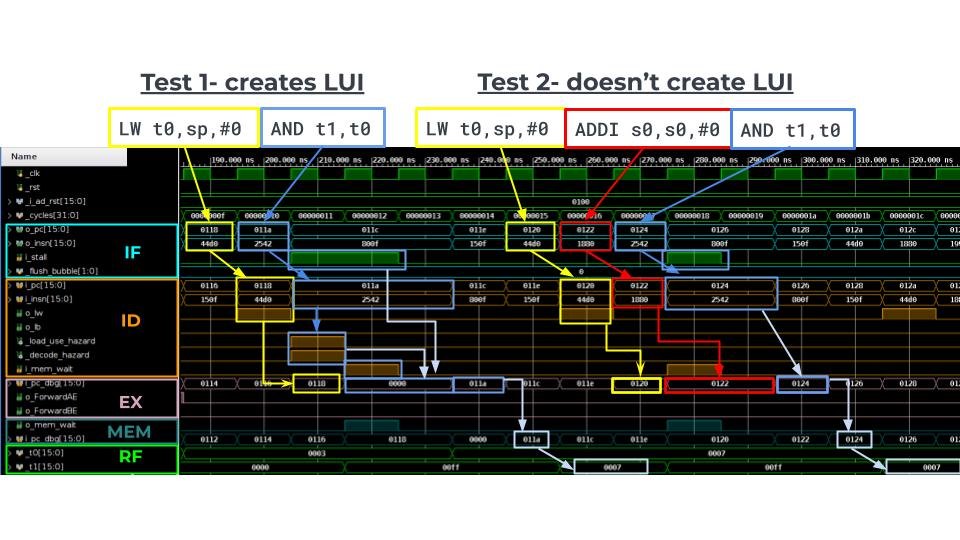
\includegraphics[width=\linewidth]{../docs/pipeline/prints_sim/behavioral_lui.jpg}
{\small Behavioral simulation\par}
\end{minipage}
\hfill
\begin{minipage}{0.48\linewidth}
\centering
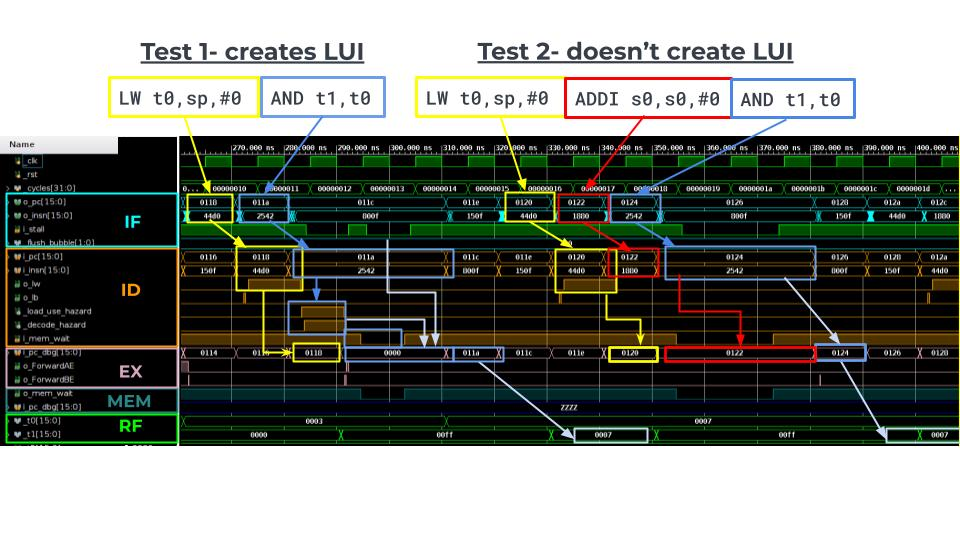
\includegraphics[width=\linewidth]{../docs/pipeline/prints_sim/postimpl_LUI.jpg}
{\small Post-implementation simulation\par}
\end{minipage}
\caption{Waveforms for a true load-use pair and for a one-instruction-gap case.}
\end{figure}

\subsection{Memory handshake stalls}

The MEM stage introduces a different kind of hazard: not a producer-consumer dependency, but variable completion latency on the data side. This hazard arises when an EX-issued load or store reaches MEM and the external data interface is not yet ready to complete the operation. In that case the pipeline must stop younger work from overtaking the in-flight memory access.

The implementation in \path{srcs/m_mem_stage.v} expresses that condition as \texttt{o\_mem\_wait}. The hazard unit turns that signal into a full upstream freeze: IF stops advancing the PC, IF/ID holds its contents, and both ID/EX and EX/MEM are frozen through \texttt{o\_stall\_ex}. Unlike the load-use case, no bubble is inserted here, because the instruction already occupying EX/MEM must remain visible to MEM until the transaction finishes.

At the SoC level, the current BRAM integration makes that behavior observable for loads. In \path{srcs/m_soc.v}, \texttt{\_mem\_rdy} is delayed by one cycle for \texttt{LW/LB}, so a core load consumes one address cycle and one completion cycle on the data side. Stores use the same handshake wires but, in the current SoC integration, do not incur that extra ready delay.

\subsection{Control hazards}

Control hazards arise when the sequential fetch stream turns out to be wrong. In this design, that happens in two ways: a BX or JAL redirects the PC from the ID stage, or an interrupt is accepted and vectors control to \texttt{i\_irq\_vector}. Because branch resolution occurs in ID rather than EX, the younger wrong-path work is concentrated at the front of the pipeline rather than several stages later.

The hazard unit therefore flushes the youngest affected state rather than indiscriminately clearing the whole machine. IF/ID is flushed on any committed branch redirect or accepted interrupt. ID/EX is flushed on interrupt acceptance and on load-use bubble insertion, but not on an ordinary taken branch. That distinction is important: when a branch resolves in ID, the older instruction already in EX is still on the correct path and must be allowed to complete normally.

The IF stage adds one more practical effect on top of the register flushes. On a redirect, \path{srcs/m_if_stage.v} loads \texttt{\_flush\_bubble <= 2'd2}; since \texttt{o\_valid} is asserted only when that counter is zero, the IF stage suppresses two later valid outputs while the redirect drains through the fetch alignment logic. In other words, the visible control-hazard cost is not just the IF/ID flush itself, but also the two invalid IF-valid opportunities that follow the redirect if the instruction side continues to hit.

\subsection{Condition-code and carry dependencies}

The active pipeline does not stall on condition-code or carry dependencies. Instead of maintaining a separate clocked PSW stage and interlocking on it, \path{srcs/m_cpu.v} derives \texttt{\_ccz}, \texttt{\_ccn}, \texttt{\_ccc}, \texttt{\_ccv}, and \texttt{\_c} combinationally from the current EX-stage outputs \texttt{\_ex\_new\_*} and \texttt{\_ex\_carry\_we}. The ID stage therefore observes EX-generated status information in the same cycle through direct combinational feedback.

This behavior is explicit in the RTL. The design avoids a dedicated CC/carry interlock, but it also means that status visibility is defined by this specific combinational path rather than by a staged PSW register.

\section{Interrupt Semantics}

Interrupt entry is integrated into the pipeline control path. The hazard unit accepts an interrupt only when \texttt{\_accept\_irq = i\_irq\_take \& \string~i\_mem\_wait}.

When \texttt{\_accept\_irq} is asserted, the CPU:
\begin{itemize}
    \item writes \texttt{PC-2} into \texttt{r14};
    \item redirects the PC to \texttt{i\_irq\_vector};
    \item clears the global interrupt enable latch;
    \item clears any in-flight \texttt{IMM} prefix state.
\end{itemize}

The CPU also edge-latches the IRQ request. A level-sensitive interrupt therefore produces one acceptance pulse per assertion interval, not one acceptance pulse per cycle.

Interrupt acceptance has explicit priority over branch commit. The CPU defines \texttt{\_id\_fire = \_ifid\_valid \& \string~\_stall\_id \& \string~\_accept\_irq} and \texttt{\_branch\_take\_commit = \_id\_branch\_take \& \_id\_fire}. If a branch is present in ID in the same cycle as interrupt acceptance, the branch does not commit.

\section{Validation}

This report includes only testbenches that compile against the active stage-based core. Each bench listed below was rebuilt and rerun against the current source set. Table~\ref{tab:validation} summarizes the coverage relevant to the pipeline control path.

\begin{longtable}{@{}p{0.36\linewidth}p{0.66\linewidth}@{}}
\caption{Validation benches used by this report.}\label{tab:validation}\\
\toprule
Bench & Property confirmed \\
\midrule
\endfirsthead

\toprule
Bench & Property confirmed \\
\midrule
\endhead

\bottomrule
\endfoot

\texttt{tb\_pipe\_branch\_flush} & Taken branch flushes younger work and preserves the architected result of the branch path. \\
\texttt{tb\_pipe\_branch\_memwait\_defer} & A branch present in ID does not commit while MEM is stalled. \\
\texttt{tb\_pipe\_mem\_wait\_freeze} & \texttt{mem\_wait} freezes the PC and the upstream pipeline state. \\
\texttt{tb\_pipe\_r0\_load\_no\_hazard} & A load targeting \texttt{r0} does not create a false dependency stall. \\
\texttt{tb\_pipe\_imm\_prefix\_flush}, \texttt{tb\_pipe\_imm\_prefix\_irq\_clear} & Prefix state is cleared correctly by redirects and by interrupt entry. \\
\texttt{tb\_pipe\_irq\_branch\_priority} & Interrupt acceptance suppresses a simultaneous branch commit. \\
\texttt{tb\_pipe\_irq\_mem\_wait\_deferral} & Interrupt acceptance is deferred until \texttt{mem\_wait} drops. \\
\texttt{tb\_pipe\_irq\_oneshot\_level} & Level-sensitive IRQ input is accepted once per assertion interval. \\
\texttt{tb\_pipe\_irq\_precise\_boundary} & Interrupt entry saves \texttt{r14} and asserts in-IRQ state at the precise pipeline boundary. \\
\texttt{tb\_pipe\_fuzz\_invariants} & No X-propagation on PC or data address and no illegal \texttt{accept\_irq \& mem\_wait} combination in bounded randomized execution. \\
\end{longtable}

\section{Load-Use Interlock and AGI Pipelines}

Golden and Mudge define the \emph{load-use interlock} (LUI) pipeline as the classical five-stage RISC organization in which load hazards are handled by an interlock and address-generation hazards do not occur. They define the \emph{address-generation interlock} (AGI) pipeline as a rearranged organization that removes the load-use hazard by moving address generation later, at the cost of address-generation interlocks and later branch resolution.\cite{goldenmudge}

\begin{table}[H]
\caption{Trade-offs between LUI-style and AGI-style organizations for this core.}
\centering
\begin{tabularx}{\linewidth}{@{}>{\ttfamily}lXX@{}}
\toprule
Style & Pros & Trade-offs \\
\midrule
LUI-style (implemented) & Keeps address generation in EX and uses an explicit load-use interlock; fits the current ID-stage control-flow resolution and verified hazard/forwarding contracts. & True load-use pairs still incur an interlock bubble; load-use latency is managed rather than structurally removed. \\
AGI-style & Can remove the classical load-use hazard by moving address generation later in the pipeline. & Introduces address-generation interlocks, tends to move branch effects later, and requires a substantial repartitioning of this core's stage and control contracts. \\
\bottomrule
\end{tabularx}
\label{tab:lui_agi_tradeoffs}
\end{table}

The pipeline implemented in this repository is not an AGI pipeline. Address generation still occurs in EX, the load-use interlock is explicit in the hazard unit, and the memory interface still occupies a later stage.

This project therefore adopts the LUI-style organization because it matches the existing RTL partition (address generation in EX, ID-stage control-flow resolution, and explicit hazard interlocks) and preserves the validated control behavior.

The active design differs from the classical LUI pipeline in one specific way: it collapses WB into MEM. The reduction in stage count comes from removing the standalone writeback stage, not from moving address generation after cache access.\cite{goldenmudge}

\section{Conclusion}

The implemented processor is a four-stage in-order pipeline with separate instruction and data memories, MEM-integrated writeback, EX/MEM operand forwarding, explicit load-use interlocking, ID-stage branch resolution, and precise interrupt entry.

The implementation details that determine latency and hazard behavior are:
\begin{itemize}
    \item one explicit forwarding source, EX/MEM to EX;
    \item write-first register-file visibility from MEM to ID in the same cycle;
    \item one decode bubble for a true load-use hazard plus one data-side ready cycle for BRAM loads;
    \item two suppressed IF-valid opportunities after a taken redirect;
    \item combinational EX-to-ID condition-code feedback in place of a registered PSW interlock.
\end{itemize}

In the terminology of Golden and Mudge, this processor remains a load-use interlock design. Its shorter depth is obtained by eliminating the explicit WB stage while preserving address generation in EX and maintaining interlocked handling of true load-use dependencies.\cite{goldenmudge}

\newpage
\begin{thebibliography}{99}

\bibitem{simplemips}
A. P. Shanthi,
\newblock ``Simple Operation of MIPS,''
\newblock University of Maryland.
\newblock \url{https://www.cs.umd.edu/users/meesh/411/SimpleMips.htm}.

\bibitem{stanfordhazards}
C. Kozyrakis,
\newblock ``Pipeline Hazards,'' EE108B Lecture 9,
\newblock Stanford University.
\newblock \url{https://web.stanford.edu/class/archive/ee/ee108b/ee108b.1082/handouts/lect.09.PipelinedHazards.pdf}.

\bibitem{cornellhazards}
Cornell CS3410 course notes,
\newblock ``Hazards I,''
\newblock Cornell University.
\newblock \url{https://www.cs.cornell.edu/courses/cs3410/2014sp/lecture/09-hazards-i-g-notes.pdf}.

\bibitem{umddh}
University of Maryland course material,
\newblock ``Dealing with Data Hazards,''
\newblock \url{https://www.cs.umd.edu/~meesh/411/mips-pipe/proj-fall11/mips-doc/node7.html}.

\bibitem{goldenmudge}
M. Golden and T. Mudge,
\newblock ``Comparison of two common pipeline structures,''
\newblock \emph{IEE Proceedings -- Computers and Digital Techniques}, vol. 143, no. 3, pp. 161--167, 1996.

\end{thebibliography}

\end{document}
